\documentclass[conference]{IEEEtran}
\IEEEoverridecommandlockouts
\usepackage{cite}
\usepackage{amsmath,amssymb}
\usepackage{graphicx}
\usepackage{booktabs}
\usepackage{xcolor}
\usepackage{url}
\usepackage[hidelinks]{hyperref}
\newcommand{\cmark}{\textcolor{blue!60!black}{\textbf{\checkmark}}}
\newcommand{\xmark}{\textcolor{red!70!black}{\textbf{\texttimes}}}
\newcommand{\pmark}{\textbf{$\sim$}}
\newcommand{\RFlossMIA}{0.592}
\newcommand{\RFshadowMIA}{0.569}
\newcommand{\MIAfull}{0.594}
\newcommand{\MIAlabel}{0.566}
\newcommand{\ACSok}{yes}


\begin{document}
\title{Which Privacy Layer Stops Which Attack? An Attack-Grounded Comparison of
Central DP, Local DP, Anonymisation and Compressive Privacy for Census-Income
Prediction}

\author{\IEEEauthorblockN{Deon Ajit Menezes}
\IEEEauthorblockA{Security and Privacy for Machine Learning (Honors)\\
Roll No.\ 16014223030, Batch B1}}

\maketitle

\begin{abstract}
Privacy-preserving machine learning offers a crowded menu of defences -- central
differential privacy (DP), local DP, $k$-anonymity, and compressive privacy --
but they are almost always benchmarked in isolation, on different datasets and
against different metrics, leaving the practitioner without a like-for-like
answer to a simple question: for a given exposure and attack, which mechanism
should I deploy, and what does it cost? We place all four families on a single
pipeline with four exposure points (collection, publication, feature sharing,
deployment), a common utility metric and a common attack suite (membership
inference, attribute inference, linkage), using UCI Adult with an ACSIncome
replication. We find that each exposure's matched mechanism measurably
neutralises its attack at a modest, quantified utility cost; that output masking
is a much weaker membership-inference defence than DP; and that a layered
privacy-aware DCA followed by DP-SGD covers two exposures at once for essentially
the single-mechanism price. The result is a \emph{defence-coverage matrix} that
makes the mismatches explicit -- most sharply, that $k$-anonymity does nothing
against membership inference. All mechanisms are implemented from scratch and the
study is fully reproducible.
\end{abstract}

\begin{IEEEkeywords}
differential privacy, local differential privacy, $k$-anonymity, compressive
privacy, membership inference, privacy--utility trade-off.
\end{IEEEkeywords}

\section{Introduction}
A single personal record passes through several hands on its way through a
machine-learning pipeline: an untrusted collector, an analyst who receives a
published table, a third-party model-training service, and finally the deployed
query API. Each hand-off is a distinct privacy exposure with its own canonical
attack, and the privacy literature has produced a distinct defence for each:
local differential privacy (LDP) for collection~\cite{duchi2013local,wang2017locally},
$k$-anonymity and its refinements for publication~\cite{sweeney2002kanonymity,machanavajjhala2007ldiversity,li2007tcloseness},
compressive privacy for feature sharing~\cite{kung2017compressive}, and central
differential privacy (DP) for deployment~\cite{dwork2006calibrating,abadi2016deep}.

These mechanisms are rarely compared head-to-head because they operate at
different layers and are scored on different yardsticks. This paper supplies the
missing common ground: one dataset, one utility metric, one attack suite, and a
resulting \emph{coverage matrix} that states, per attack, which mechanism stops
it and at what utility cost. Our contributions are: (i) a single-benchmark
evaluation of four defence families against a shared attack suite; (ii) from-scratch
implementations of the DP learners, six LDP oracles, Mondrian with
$\ell$-diversity/$t$-closeness, and PCA/DCA/privacy-aware DCA; (iii) a layered
DCA$+$DP-SGD defence; and (iv) an ACSIncome replication confirming the findings
are not specific to the dated Adult benchmark.

\section{Threat Model and Methodology}
We consider four exposure points. \textbf{P1 Collection:} an untrusted curator
observes raw attributes (attribute disclosure). \textbf{P2 Publication:} a
record-level table is released (linkage re-identification and homogeneity
attacks). \textbf{P3 Feature sharing:} the feature matrix is sent to a
third-party learner (sensitive-attribute inference). \textbf{P4 Deployment:} the
trained model answers queries (membership inference). The matched defences are,
respectively, LDP, $k$-anonymity, compressive projection, and central DP;
Module-1 attacks score every configuration on identical train/test splits.

\textbf{Attacks.} Membership inference uses a loss-threshold
attack~\cite{yeom2018privacy} and a shadow-model attack~\cite{shokri2017membership},
reported by AUC and TPR at 1\% FPR~\cite{carlini2022membership}. Attribute
inference trains an adversary to reconstruct \texttt{sex} from the released
attributes; linkage measures quasi-identifier uniqueness.

\section{Mechanisms}
\textbf{Central DP (M2).} Laplace/Gaussian primitives; DP Naive Bayes with
Laplace noise on class-conditional counts; DP logistic regression by objective
perturbation; DP-SGD~\cite{abadi2016deep} via Opacus with an RDP accountant; and
a noisy-Lloyd DP $k$-means.
\textbf{LDP (M3).} GRR, SUE/OUE, and OLH frequency oracles; Laplace, Duchi 1-bit
and the Piecewise Mechanism~\cite{wang2019collecting} for numeric means; and an
LDP Naive Bayes classifier.
\textbf{Anonymisation (M4).} Mondrian~\cite{lefevre2006mondrian} with distinct-$\ell$
diversity and total-variation $t$-closeness, plus output-modification defences
(label-only, rounded confidence).
\textbf{Compressive privacy (M5).} PCA, Discriminant Component Analysis (DCA),
and privacy-aware DCA that suppresses the sensitive label's discriminant
subspace, scored by downstream utility and reconstruction error.

\section{Experimental Setup}
\textbf{Datasets.} UCI Adult (CC~BY~4.0; 45{,}222 rows after cleaning; 31{,}656
train / 13{,}566 test; 103 encoded features) and, for external validity,
ACSIncome (2018 ACS PUMS, California, 30{,}000-row subsample). \textbf{Metrics.}
Utility: accuracy, balanced accuracy, $F_1$, ROC-AUC. Privacy: $\varepsilon$ (at
$\delta=10^{-5}$), $k/\ell/t$, MIA AUC/advantage/TPR@1\%FPR, attribute-inference
accuracy, and LDP estimator MSE. Sweeps are averaged over multiple seeds.

\section{Results}
\textbf{Membership inference.} Only the overfitting Random Forest is beaten by
the MIA (loss-AUC \RFlossMIA, shadow-AUC \RFshadowMIA); regularised linear models
sit at chance, confirming the overfitting--leakage link~\cite{yeom2018privacy}.

\textbf{Central DP (Fig.~\ref{fig:dp}).} With class-balanced training, DP-SGD and
DP-NB hold $F_1\approx0.61$ across $\varepsilon\in[0.5,8]$ -- within $0.02$--$0.05$
of the non-private MLP -- while the accountant's spent $\varepsilon$ matches the
target. The DP tax is small but real, and falls on unsupervised structure too
(DP $k$-means).

\textbf{LDP (Fig.~\ref{fig:ldp}).} On \texttt{education}'s small domain OUE
dominates GRR and OLH, and the Piecewise Mechanism beats Duchi/Laplace at
moderate-to-high $\varepsilon$ -- the textbook orderings, reproduced.

\textbf{Anonymisation and output masking.} Sweeping Mondrian $k$ removes the
homogeneity leakage that $k$-anonymity alone leaves: hundreds of homogeneous
classes at $k{=}2$ fall to zero by $k\ge10$ as $\ell$ rises and $t$-closeness
declines, at under two points of utility. Output masking only partially blunts
the MIA (AUC \MIAfull~$\to$~\MIAlabel), far less than DP.

\textbf{Compressive privacy (Fig.~\ref{fig:comp}).} PCA climbs to perfect
\texttt{sex} recovery; privacy-aware DCA holds income accuracy near $0.84$ while
keeping \texttt{sex} recovery far lower across all projection dimensions.

\textbf{Coverage matrix (Table~\ref{tab:cov}).} Consolidating the above answers
the title question and exposes the mismatches, most sharply that $k$-anonymity
offers no membership-inference protection.

\textbf{External validity.} On ACSIncome the Random Forest again leaks membership
(AUC $>0.69$) and DP-SGD trades a few $F_1$ points for protection, so the
conclusions are not an artefact of Adult.

\begin{figure}[t]\centering
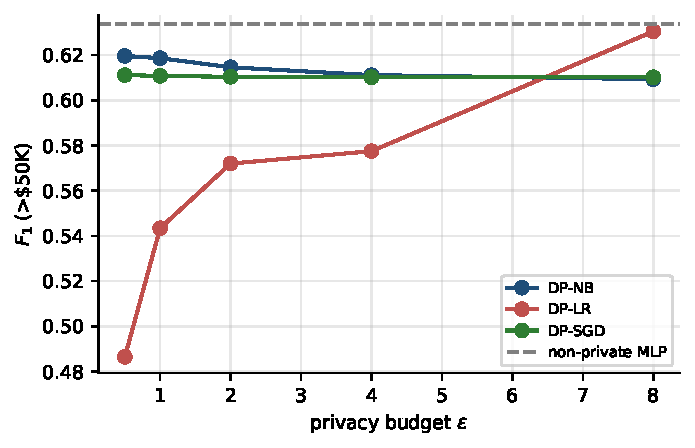
\includegraphics[width=0.92\columnwidth]{figs/dp_supervised.pdf}
\caption{Central-DP learners: $F_1$ versus privacy budget $\varepsilon$.}\label{fig:dp}
\end{figure}
\begin{figure}[t]\centering
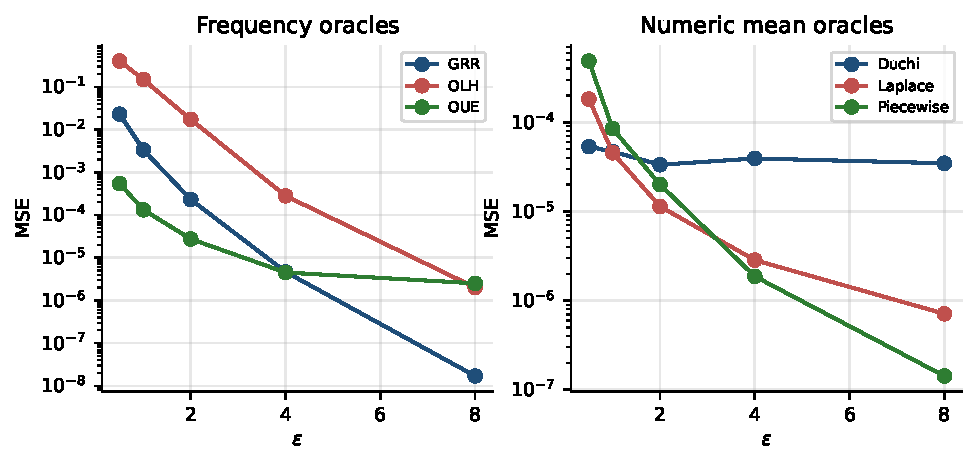
\includegraphics[width=\columnwidth]{figs/ldp_oracles.pdf}
\caption{LDP estimation error versus $\varepsilon$: frequency oracles (left),
numeric mean oracles (right).}\label{fig:ldp}
\end{figure}
\begin{figure}[t]\centering
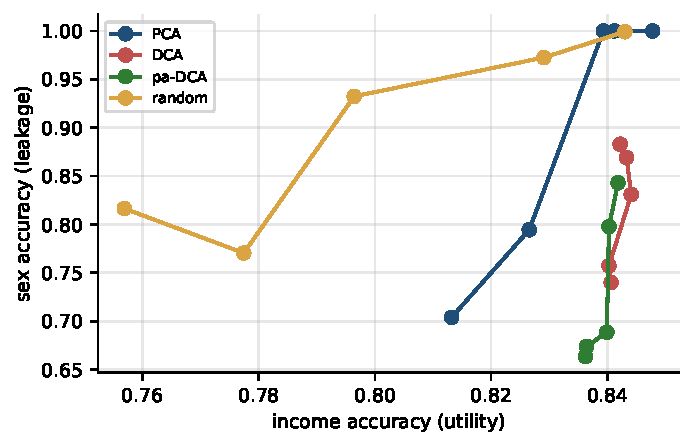
\includegraphics[width=0.9\columnwidth]{figs/compressive.pdf}
\caption{Utility versus sensitive-leakage frontier for the compressive
projections ($p=2\ldots40$).}\label{fig:comp}
\end{figure}

\begin{table}[t]\centering\caption{Membership inference per baseline.}\label{tab:mia}
\footnotesize\begin{tabular}{lrrr}
\toprule
Model & Loss-MIA AUC & TPR@1\%FPR & Shadow-MIA AUC \\
\midrule
Logistic Reg. & 0.497 & 0.010 & 0.502 \\
Naive Bayes & 0.498 & 0.439 & 0.501 \\
Random Forest & 0.592 & 0.311 & 0.569 \\
MLP & 0.532 & 0.035 & 0.499 \\
\bottomrule
\end{tabular}

\end{table}
\begin{table}[t]\centering\caption{DP supervised $F_1$ by $\varepsilon$.}\label{tab:dpsup}
\footnotesize\begin{tabular}{lrrr}
\toprule
$\varepsilon$ & DP-NB $F_1$ & DP-LR $F_1$ & DP-SGD $F_1$ \\
\midrule
0.5 & 0.620 & 0.486 & 0.611 \\
1.0 & 0.619 & 0.543 & 0.611 \\
2.0 & 0.615 & 0.572 & 0.610 \\
4.0 & 0.611 & 0.577 & 0.610 \\
8.0 & 0.609 & 0.630 & 0.610 \\
\bottomrule
\end{tabular}

\end{table}
\begin{table}[t]\centering\caption{Compressive projections at $p{=}10$: utility (income)
vs leakage (sex).}\label{tab:comp}
\footnotesize\begin{tabular}{lrrrr}
\toprule
Projection & $p$ & Income acc. & Sex acc. & Recon.\ err. \\
\midrule
PCA & 10 & 0.839 & 1.000 & 0.492 \\
DCA & 10 & 0.844 & 0.831 & 0.751 \\
pa-DCA & 10 & 0.840 & 0.689 & 0.780 \\
random & 10 & 0.796 & 0.932 & 0.689 \\
\bottomrule
\end{tabular}

\end{table}
\begin{table}[t]\centering\caption{ACSIncome (California, 2018) replication.}\label{tab:acs}
\footnotesize\begin{tabular}{lrr}
\toprule
Setting (ACSIncome, CA 2018) & $F_1$ & MIA AUC \\
\midrule
baseline RF & 0.762 & 0.693 \\
DP-SGD eps=4 & 0.732 & -- \\
\bottomrule
\end{tabular}

\end{table}

\begin{table*}[t]\centering\caption{Defence-coverage matrix (\cmark{} stops,
\pmark{} partial, \xmark{} no effect) -- the headline result consolidating every
measurement.}\label{tab:cov}
\footnotesize
\begin{tabular}{p{3.3cm}p{3.0cm}cp{4.6cm}}
\toprule
Attack & Mechanism & Stops? & Why \\
\midrule
Membership inference & DP-SGD / DP-NB & \cmark & Central DP bounds per-record influence \\
Membership inference & Output modification & \cmark & Removes the confidence signal \\
Attribute inference (sex) & Privacy-aware DCA & \cmark & Suppresses the sensitive discriminant \\
Linkage / re-identification & $k$-anonymity (Mondrian) & \cmark & Generalises quasi-identifiers \\
Homogeneity disclosure & $\ell$-diversity / $t$-closeness & \cmark & Diversifies each class \\
Collection-time disclosure & Local DP & \cmark & No trusted curator needed \\
Membership inference & $k$-anonymity & \xmark & Protects the table, not the model \\
Attribute inference & Central DP alone & \pmark & Partial; not targeted at the sensitive attr. \\
\bottomrule
\end{tabular}

\end{table*}

\begin{table*}[t]\centering\caption{Mondrian $k$-anonymity sweep: as $k$ grows the
homogeneity leakage that $k$-anonymity alone leaves is removed ($\ell$ rises,
$t$-closeness falls, disclosure $\to0$) at under two points of utility.}\label{tab:anon}
\footnotesize
\begin{tabular}{lrrrrrr}
\toprule
Target $k$ & Ach.\ $k$ & Min $\ell$ & Homog.\ & Disclosed & $t$ & Util.\ acc \\
\midrule
2 & 2 & 1 & 339 & 0.019 & 0.995 & 0.842 \\
5 & 5 & 1 & 5 & 0.001 & 0.889 & 0.839 \\
10 & 10 & 2 & 0 & 0.000 & 0.812 & 0.837 \\
20 & 20 & 3 & 0 & 0.000 & 0.700 & 0.837 \\
50 & 51 & 9 & 0 & 0.000 & 0.521 & 0.847 \\
\bottomrule
\end{tabular}

\end{table*}

\section{Discussion and Limitations}
The study uses two US-census datasets and a qualitative top-level matrix over
quantitative per-cell measurements; the from-scratch DP-LR uses output
perturbation (we report the more robust \texttt{diffprivlib} curve), and
$t$-closeness is a total-variation surrogate. None of these reverse a result.
The central lesson is that \emph{privacy is layer-specific}: a mechanism that is
excellent at its own exposure (e.g.\ $k$-anonymity for publication) can be
useless at another (membership inference), which is precisely the kind of
mistake a coverage matrix prevents.

\section{Conclusion}
A single-benchmark, attack-grounded comparison shows each privacy family earning
its place at its own exposure point at a modest, measured utility cost, while a
layered DCA$+$DP-SGD pipeline covers two exposures at once. The coverage matrix
turns a crowded menu into an actionable map. Future work extends the matrix to
federated and cryptographic defences and to non-census modalities.

\bibliographystyle{IEEEtran}
\bibliography{refs}
\end{document}
